\chapter{Introduction} \label{chap:intro}


%###############################################################################################################################
%###############################################################################################################################
%###############################################################################################################################
\section{Nuclear Fusion}%
\label{sec:intro_whatisfusion}

Nuclear fusion is a reaction which combines multiple light nuclei together into heavier nuclei.
If the products of the reaction are more tightly bound than the reactants, excess energy is also released to the products.
Broadly, the binding energy per nucleon of common nuclear isotopes increases with atomic mass up to iron, ${}^{56}\text{Fe}$, and decreases afterwards, as is shown in Fig.~\ref{fig:intro_BEperNucleon}.
The reverse process, nuclear fission, operates by splitting heavy nuclei into lighter products, thus energy is released via fusion by combining elements up to iron and via fission down to iron.
In 2023, fission made up approximately 9.1\% of the global electricity mix~\cite{ember_institute_statistical_2024}.
Like fission, fusion energy would be carbon free at the point of production, but it would also offer further distinct advantages.
Fusion power plants would not produce energy via potentially dangerous chain reactions and would generate little-to-no long-lived nuclear waste, depending on the specific fuel that was used.
In comparison with other low-carbon power sources, including wind and solar, studies have shown that fusion energy could have a competitive \ac{LCOE}, which is a metric that compares the economic costs of a power plant over its lifetime to the value of energy produced~\cite{griffiths_commercialisation_2022}.
Performing controlled nuclear fusion on Earth for energy production has been an active area of research for many decades and many significant scientific and engineering challenges remain to be resolved, in order to make it a viable energy source.

The likelihood of two reactants undergoing a specific fusion reaction is described by the cross-section of the interaction,
\begin{equation}
    \label{eq:intro_cross_sec}
    \sigma(E) = \frac{S(E)}{E} e^{-E_G/E},
\end{equation}
which is a function of the centre of mass energy, $E$, the `astrophysical $S$-factor', $S(E)$, which is a weakly varying function of energy for many typically deployed reactants and the Gamow Energy, $E_G$~\cite{atzeni_physics_2004}.
The exponential term in Eq.~\ref{eq:intro_cross_sec} is related to the probability of reactants tunnelling through the energy barrier, due to electrostatic Coulomb repulsion.
One approach to achieving the energies required to overcome this barrier are `beam-target' configurations, wherein a high energy beam of reactants is focussed onto a stationary target, has proven unviable~\cite{rider_general_1995}.
Thermonuclear fusion is the alternative approach, wherein the bulk fuel is heated to sufficient temperatures that the particles in the high-energy tail of the distribution have sufficient energy to undergo fusion reactions.
If the fusion products are able to deposit a sufficient fraction of their energy back into the fuel, then a self-sustaining fusion reaction is possible, where the high temperatures required for the reactants to fuse is maintained.
For a fusion reaction with reactants labelled by 1 and 2, the number of fusion reactions per unit time and volume is known as the `volumetric reaction rate',
\begin{equation}
    \label{eq:intro_reacrate}
    R_{12} = \frac{n_1 n_2}{1+\delta_{12}} \langle \sigma v \rangle,
\end{equation}
where $v$ is the relative velocity of a pair of reactants, $\delta_{12}$ is the Kronecker delta, which accounts for double counting of species and the `averaged reactivity' $\langle \sigma v \rangle$ is defined as the integral over the velocity distribution,
\begin{equation}
    \label{eq:intro_reactivity}
    \langle \sigma v \rangle \equiv \int_0^{\infty} \sigma(E) v f(v)\ \text{d}v.
\end{equation}
Eq.~\ref{eq:intro_reacrate} explicitly demonstrates that achieving a high fuel density, can significantly enhance reaction rates due to the square dependence.

\begin{figure}[t!]
    \includegraphics[width=0.9\linewidth]{Introduction/Images/BE_per_nucleon.png}
    \centering
    \caption{Binding energy per nucleon for common nuclear isotopes.
    Binding energy peaks close to iron, therefore energy is released for reactions which increase binding energy.
    ${}^{4}\text{He}$ has a particularly high binding energy and therefore fusion reactions which results in this isotope are strong candidates for fusion energy production.}%
    \label{fig:intro_BEperNucleon}
\end{figure}

The efficacy of a fusion fuel is dictated by the availability of the reactants, the fusion products, the averaged reactivity of the reactants and the energy released per reaction, $Q$, which is the difference in binding energy between the reactants and products.
Most current, fusion-energy experiments are focussed on demonstrating that fusion power production is possible, thus the choice of fuel is predominantly dictated by the reactivity.
Hydrogen-Hydrogen isotope fusion reactions have much higher reactivities than other elements, because the Coulomb repulsion scales as $Z^2$, thus the Gamow energy, $E_G$ is significantly smaller.


Describe main approaches to fusion on earth.

%###############################################################################################################################
%###############################################################################################################################
%###############################################################################################################################
\section{Inertial Confinement Fusion}%
\label{sec:intro_ICF}

Broadly describe the key idea of ICF here.

%################################################################################
%################################################################################
\subsection{Ignition Requirements}%
\label{sec:intro_icf_ignition}

Give Lawson ICF version.
IFE requirements.

%################################################################################
%################################################################################
\subsection{Central Hotspot Ignition}%
\label{sec:intro_centralhotspot}

\begin{figure}[t!]
    \includegraphics[width=0.7\linewidth]{Introduction/Images/hotspot ignition white.png}
    \centering
    \caption{Key Stages of the central hotspot ignition \ac{ICF} concept.
    }%
    \label{fig:intro_hotspot}
\end{figure}

Describe ablation pressure, ignite small volume of fuel etc.

%################################################################################
%################################################################################
\subsection{Alternative Approaches}%
\label{sec:intro_icf_alt}

Shock and fast ignition.

%###############################################################################################################################
%###############################################################################################################################
%###############################################################################################################################
\section{Current Experiments/ Main Approaches}%
\label{sec:intro_ICF}

Small intro on direct vs indirect.

%################################################################################
%################################################################################
\subsection{Indirect Drive}%
\label{sec:intro_indirect}

\begin{figure}[t!]
    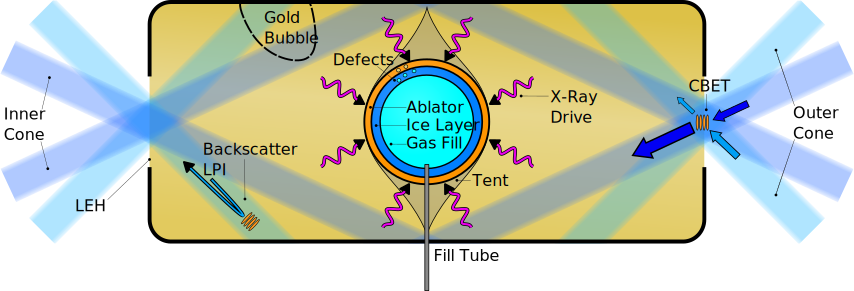
\includegraphics[width=\linewidth]{Introduction/Images/indirect icf white.png}
    \centering
    \caption{Schematic of the indirect-drive approach to \ac{ICF}.
    }%
    \label{fig:intro_indirect}
\end{figure}

Talk about all that jazz and give the diagram.
Talk about NIF and ignition, gain etc.

%################################################################################
%################################################################################
\subsection{Direct Drive}%
\label{sec:intro_direct}

\begin{figure}[t!]
    \includegraphics[width=0.7\linewidth]{Introduction/Images/direct icf white.png}
    \centering
    \caption{Schematic of the direct-drive approach to \ac{ICF}.
    }%
    \label{fig:intro_direct}
\end{figure}

Say its the assumed version for IFE.
Give a much more detailed anatomy of implosion, incl diagram.
Talk about hydro-scaled ignition etc.

%###############################################################################################################################
%###############################################################################################################################
%###############################################################################################################################
\section{Laser Interaction with Plasmas}%
\label{sec:intro_laserplasmas}

Understanding lasers is obviously crucial for Direct, indirect and hedp more generally.

%################################################################################
%################################################################################
\subsection{Regime of interest}%
\label{sec:intro_laser_regime}

Want collisional absorption and to avoid LPIs.
Therefore short wavelength, high power lasers, with limits to peak intensity.
Balance between $P_abl$ and high $I*lam^2$.

%################################################################################
%################################################################################
\subsection{ICF Relevant LPIs}%
\label{sec:intro_LPIs}

\begin{figure}[t!]
    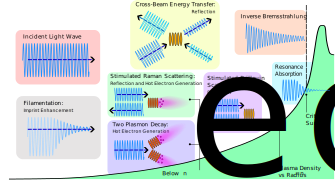
\includegraphics[width=\linewidth]{Introduction/Images/LPI diagram.png}
    \centering
    \caption{Important \ac{LPIs} for direct-drive \ac{ICF}.
    }%
    \label{fig:intro_dd_lpis}
\end{figure}

Damaging class of laser-plasma interactions for ICF.
Give diagram of how they work microphysically.
Include direct drive LPI diagram.
Introduce each in turn and say what they do for direct and indirect.

%###############################################################################################################################
%###############################################################################################################################
%###############################################################################################################################
\section{Objective of the work}%
\label{sec:intro_objective}

LPIs are important for current experiments.
Need to include models for them in integrated codes.
Also, next gen lasers will eliminate LPIs hopefully with bandwidth, so need to understand how they degrade current experiments to accurately extrapolate.
Create laser module for CHIMERA, specifically capable of modelling LPIs, and then see what their effect is for direct-drive.
